% Packages
\documentclass[12pt]{article}
\usepackage[margin=2.5cm]{geometry}
\usepackage{lipsum}
\usepackage{titlesec, titletoc}
\usepackage[svgnames, table]{xcolor}
\usepackage{algorithm}
\usepackage{algpseudocode}
\usepackage{mdframed}
\usepackage[T1]{fontenc}
\usepackage{amsmath,amsthm,amsfonts,amssymb,mathtools}
\usepackage[osf]{mathpazo}
\usepackage{enumitem}

% Formating setup
\footskip = 1 cm
\setlength{\parindent}{0pt}
\pdfpxdimen=1in
\parindent = 0pt
\definecolor{myBlue}{RGB}{0, 81, 255}
\titleformat{\section}[block]{\sffamily\large\bfseries}{\thesection}{.5em}{\textcolor{myBlue}
{\titlerule[1.5pt]}\\\sffamily}[\vspace*{-3mm}\textcolor{myBlue}{\titlerule[1.5pt]}]
\titleformat{\subsection}{\large\sffamily\bfseries}{\thesubsection}{0.5em}{\textcolor{Black}}
\newcounter{boxedlistcounter}
\newenvironment{pseudo}{%
  \setcounter{boxedlistcounter}{0}% <-- Add this line to reset the counter
  \mdframed[
    linecolor=black, % color of the border
    linewidth=1.5pt, % thickness of the border
    roundcorner=10pt, % radius of the corners
    innertopmargin=0.6\baselineskip, % space at the top of the box
    innerbottommargin=0.6\baselineskip, % space at the bottom of the box
  ]
  \fontsize{12pt}{14pt}\selectfont % add font size command here
  \mdseries % add font series command here
}{%
  \endmdframed%
}
\newcommand{\I}{\par\stepcounter{boxedlistcounter}\arabic{boxedlistcounter}.\hspace{5pt}}
\newcounter{boxedlistcounter2}
\newenvironment{Proof}{%
  \refstepcounter{boxedlistcounter2}%
  \mdframed[
    linecolor=black, % color of the border
    linewidth=1.5pt, % thickness of the border
    roundcorner=10pt, % radius of the corners
    innertopmargin=\baselineskip, % space at the top of the box
    innerbottommargin=\baselineskip, % space at the bottom of the box
  ]
  \fontsize{12pt}{14pt}\selectfont % add font size command here
  \mdseries % add font series command here
}{%
  \endmdframed%
}
\newcommand{\PI}{\par\textbullet\hspace{5pt}}
\setlist[itemize]{itemsep=1pt}
\newcommand{\NL}{\par\hspace{12.5pt}}
\setlist[itemize]{itemsep=1pt}

% Custom commands
\newcommand{\for}[1]{\textbf{for} #1 \textbf{do}}
\newcommand{\IF}[1]{\textbf{if} #1 \textbf{then}}
\newcommand{\ELIF}[1]{\textbf{else if} #1 \textbf{then}}
\newcommand{\ELSE}{\textbf{else}}
\newcommand{\return}[1]{\textbf{return} #1}
\newcommand{\assign}{ $\leftarrow$ }
\newcommand{\DEF}[2]{\textbf{def} #1(#2):}
\newcommand{\1}{\space \quad}
\newcommand{\2}{\quad \quad \quad}
\newcommand{\3}{\quad \quad \quad \quad \space}
\newcommand{\4}{\quad \quad \quad \quad \quad \quad}
\newcommand{\5}{\quad \quad \quad \quad \quad \quad \quad \space}
\newcommand{\comment}[1]{\hfill \textit{\# #1}}
\newcommand{\while}[1]{\textbf{while} #1 \textbf{do}}

% Document start ------------------------------------------------------------------------------------
\begin{document}

% Section 1  ----------------------------------------------------------------------------------------
\section{Introduction to Graphs}
A graph G is a pair (V, E), where V is a set of nodes, called vertices and E is a collection of pairs of 
vertices, called edges.

\vspace{10pt}
\textbf{Edge Types}\\
A graph can be directed or undirected. In a directed graph, the edges are ordered pairs of vertices (u, v),
where u is the origin/tail and v is the destination/head. In an undirected graph, the edges are unordered 
pairs of vertices (u,v), whereby u and v can access each other either way.

\vspace{10pt}
\textbf{Simple paths}\\
A path is a sequence/set of vertices such that every pair of consecutive vertices is connected by an edge. A simple
path is a path with no repeated vertices. As such, all vertices in that path are distinct. 

\vspace{10pt}
\textbf{Cycles in graphs}\\
A cycle is a path with at least one edge, whose first and last vertices are the same. A simple cycle is a cycle.
A simple cycle is one where all vertices are distinct, except for the first and last vertices. An acyclic graph has 
no cycle in it, which is impossible for undirected graphs. A directed graph can be acyclic.

\vspace{10pt}
\textbf{Subgraphs}\\
A subgraph S of a graph G is defined as S = (U, F) where U is a subset of vertices in V and F is a subset of edges 
in E. An induced subgraph of G is a subgraph that is formed by selecting a subset U of vertices and all the edges 
in G that have both endpoints in U, which is denoted as G[U]. Similarly, an induced subgraph can be formed by selecting 
a subset F of edges and the vertices that are endpoints of the edges in F, which is denoted as G[F].

\vspace{10pt}
\textbf{Connectivity}\\
A graph G = (V, E) is considered connected if there is a path between every pair of vertices in V. In other words, 
every vertex in the graph is reachable from every other vertex. A connected component of a graph G is a maximally connected 
subgraph of G, meaning that it is a subgraph that is connected, and there is no larger connected subgraph that contains it. 
A graph is considered disconnected if it has two or more connected components, which means that there are pairs of vertices 
that are not connected by any path in the graph.

\vspace{10pt}
\textbf{Trees and Forests}\\
An unrooted tree is a graph that is connected and has no cycles. A forest is a graph without cycles, and its connected components 
are trees. Every tree on n vertices has exactly n-1 edges, which is a well-known property of trees in graph theory. A rooted 
tree is a type of tree that is produced by a directed graph where the edges are directed away from the root.

\subsection{Graph Properties}
\begin{itemize}
  \item $\sum_{v \in V}$ deg(v) = 2m, where m is the number of edges in the graph. This states that the sum of the 
  degrees of all the vertices in the graph is equal to twice the number of edges in the graph.
  \item In a simple undirected graph m <= n (n - 1)/2.
  \item n represents the number of vertices, m represents the number of edges. And $\triangle$ represents the maximum degree.
\end{itemize}

% Section 2  ----------------------------------------------------------------------------------------
\section{Graph ADT}
We model the abstraction as a combination of three data types: Vertex, Edge, and Graph.
A Vertex stores an associated object (e.g., an airport code) that is retrieved with a getElement() method.
An Edge stores an associated object (e.g., a flight number, travel distance) that is retrieved with a getElement() method. 

\subsection{Edge List Structure}
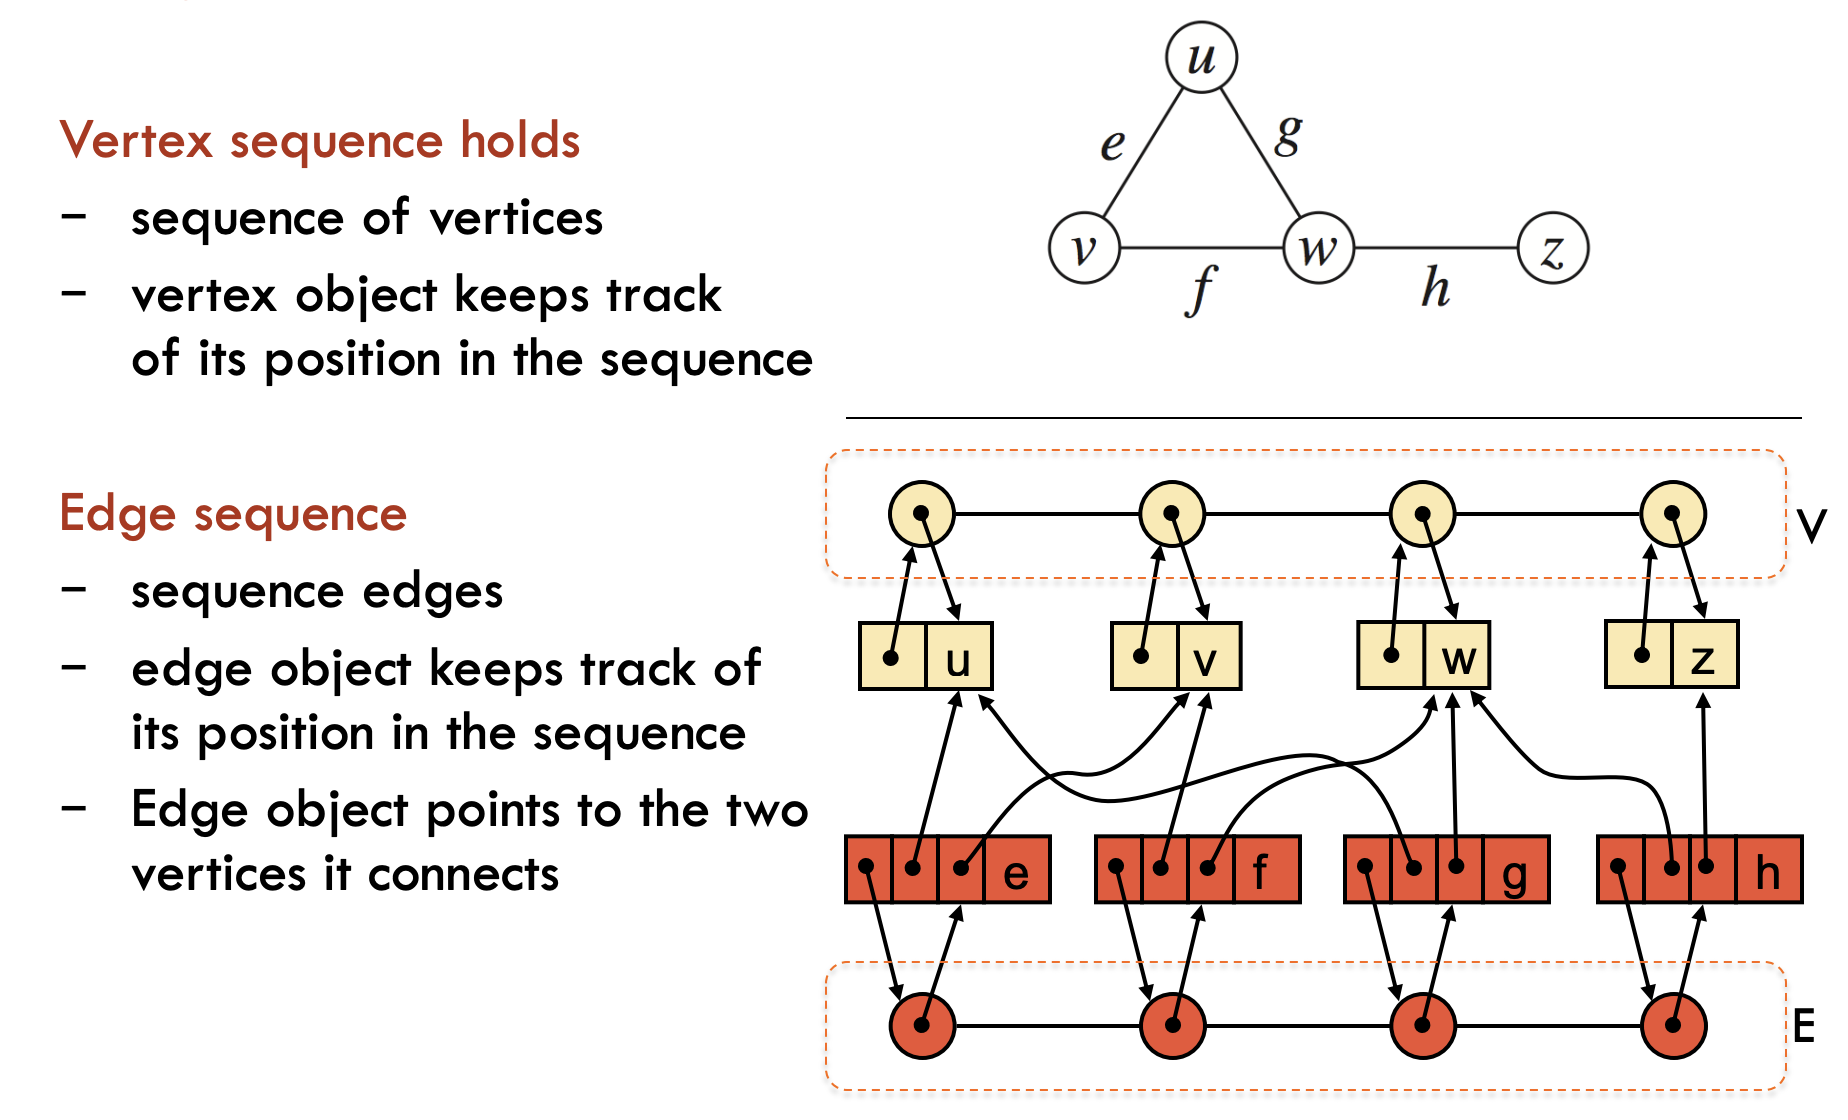
\includegraphics[width=\textwidth]{image13.png}

\subsection{Adjacency List}
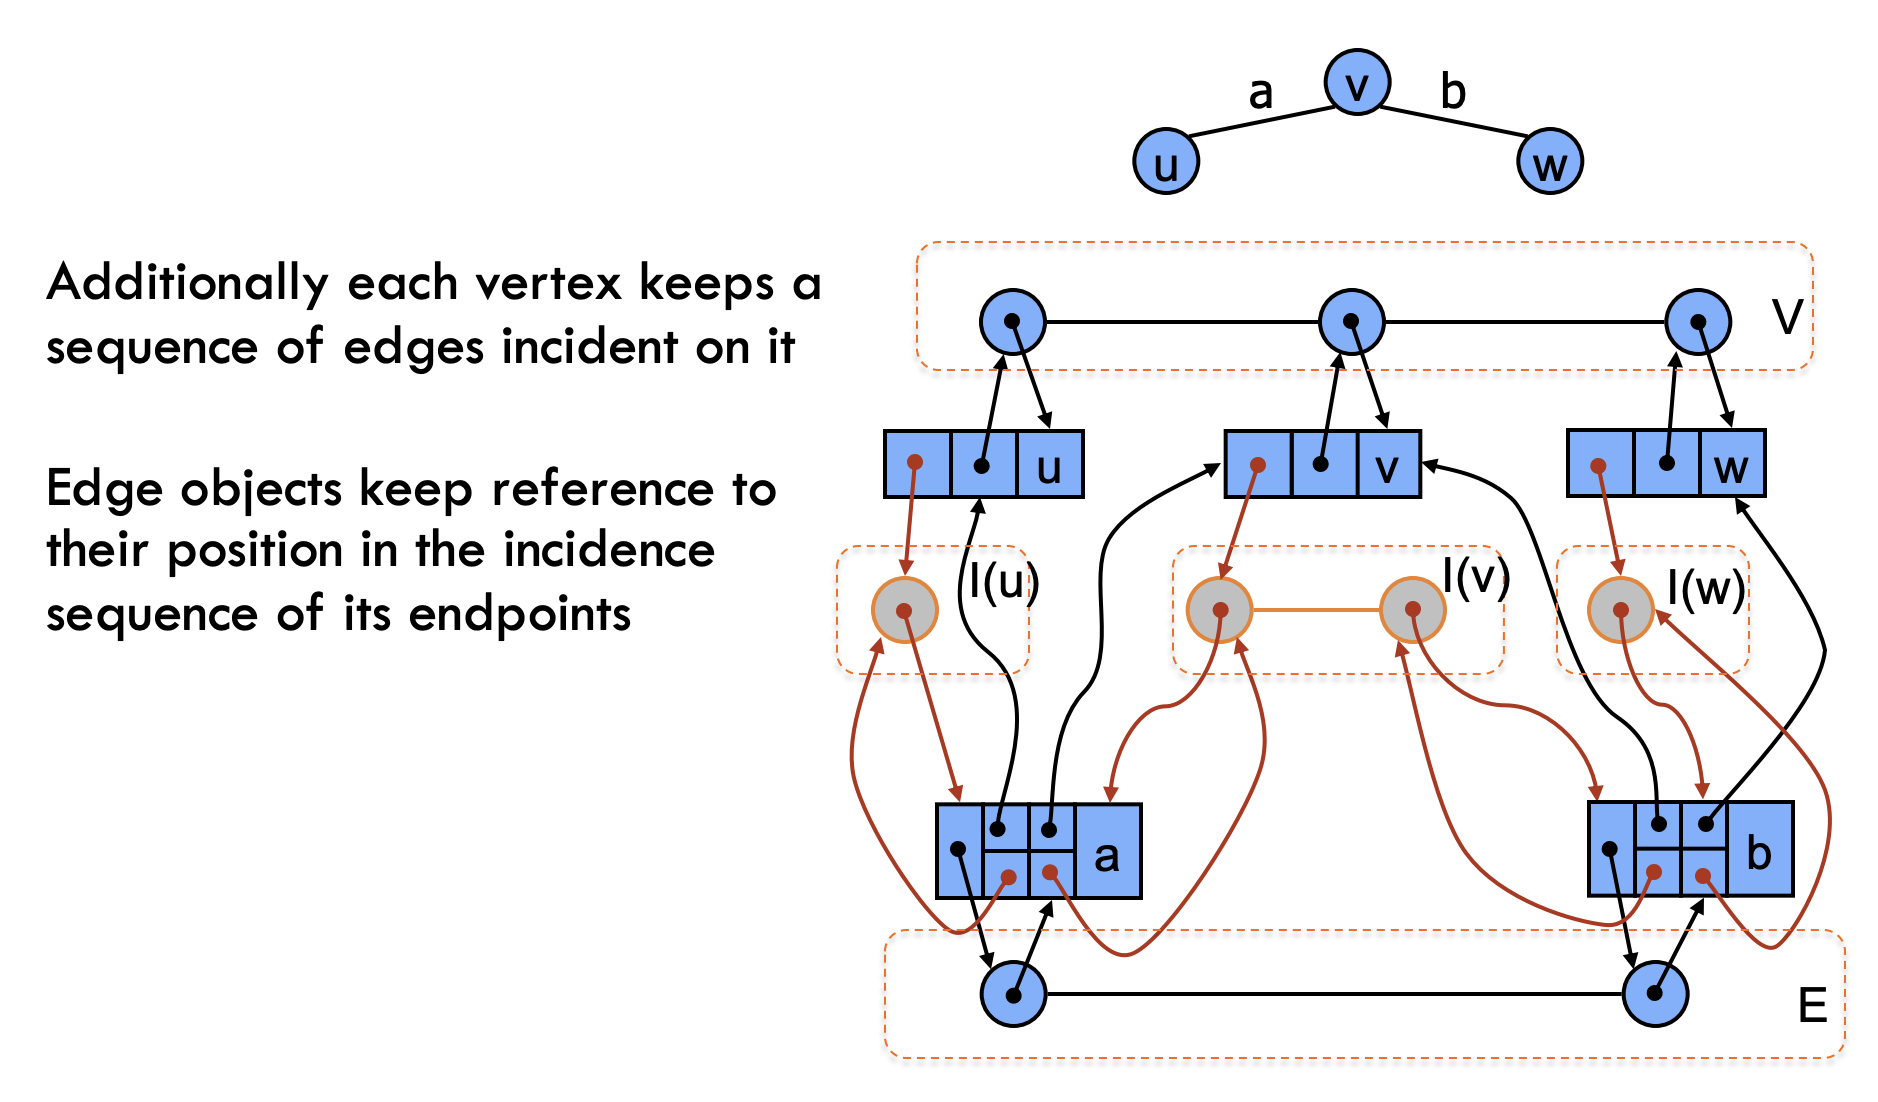
\includegraphics[width=\textwidth]{image14.png}

\subsection{Adjacency Matrix Structure}
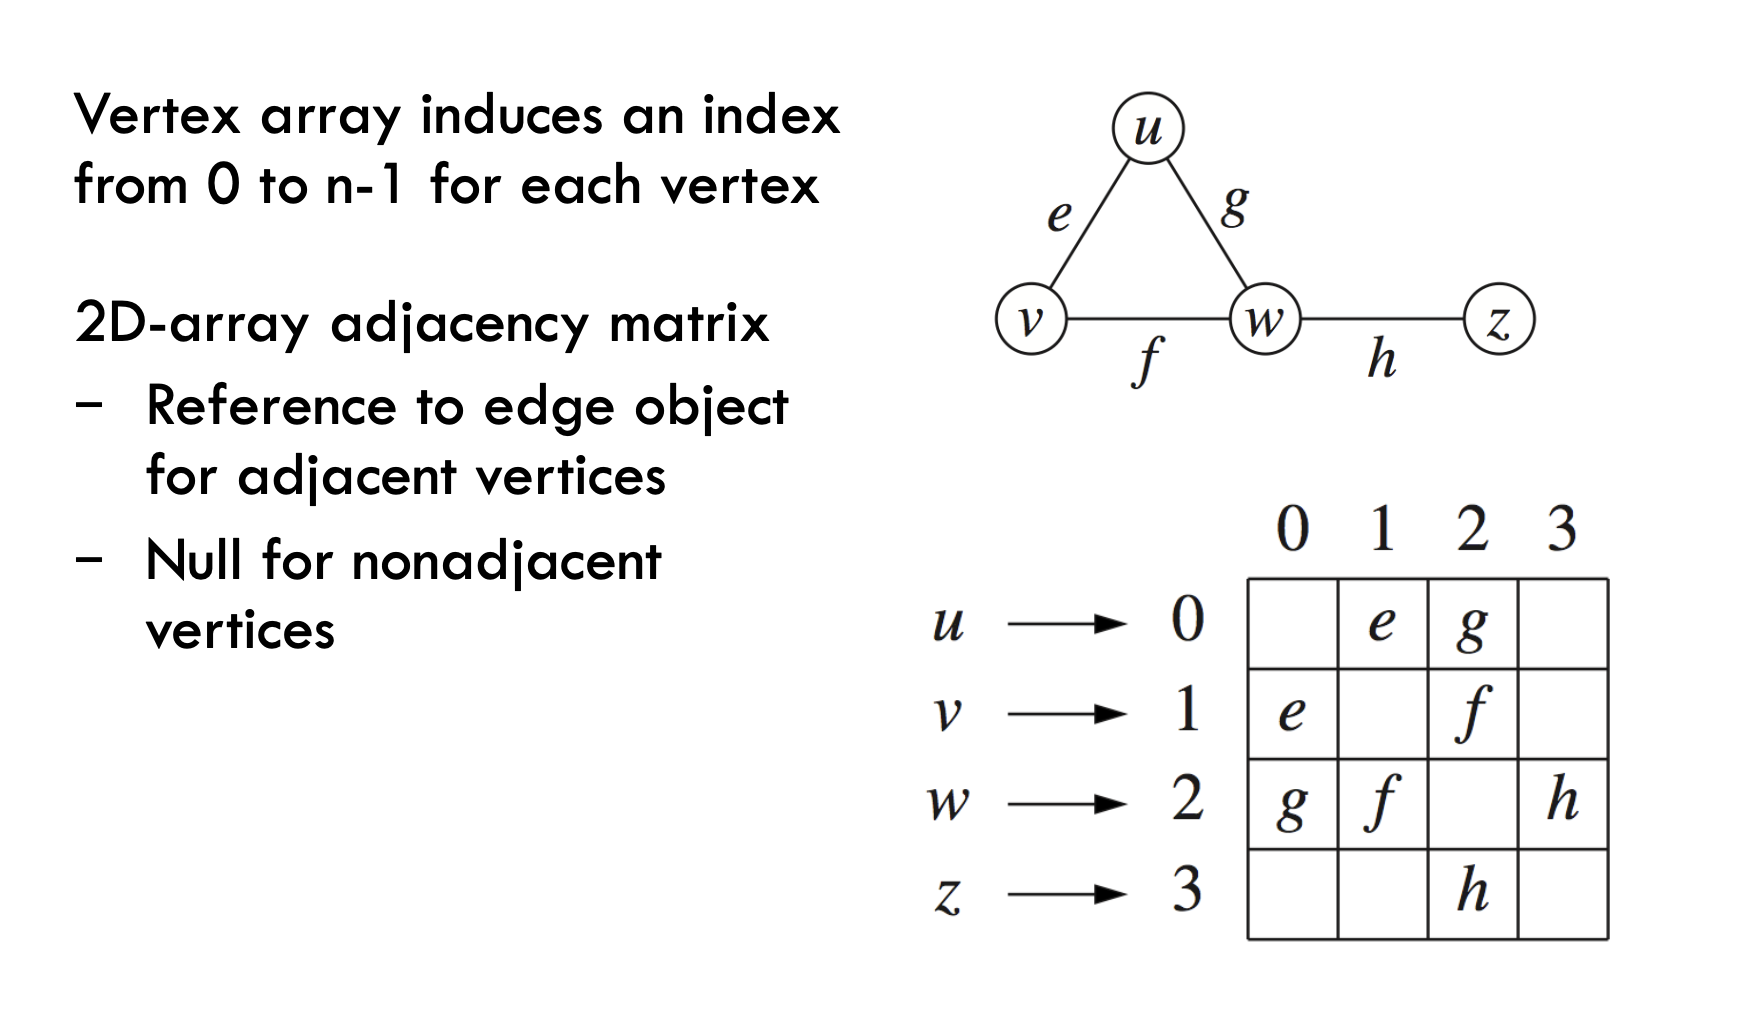
\includegraphics[width=\textwidth]{image15.png}

\subsection{Asymptotic performance}
\begin{tabular}{|l|l|l|l|}
  \hline
  \rowcolor{myBlue}
  \color{white}{\textbf{No parallel edges/s-loops}} & \color{white}{\textbf{Edge List}} & \color{white}{\textbf{Adjacency List}} & \color{white}{\textbf{Adjacency Matrix}} \\
  \hline
  Space  & O(n + m) & O(n + m) & O($n^2$) \\
  \hline
  incidentEdges(v) & O(m) & O(deg(v)) & O(n) \\
  \hline
  getEdge(u, v) & O(m) & O(min(deg(u), deg(v))) & O(1) \\
  \hline
  insertVertex(x) & O(1) & O(1) & O($n^2$)\\
  \hline
  insertEdge(u, v, x) & O(1)  & O(1)  & O(1) \\
  \hline
  removeVertex(v) & O(m) & O(deg(v)) & O($n^2$)\\
  \hline
  removeEdge(e) & O(1) & O(1) & O(1)\\
  \hline
\end{tabular}

% Section 3  ----------------------------------------------------------------------------------------
\section{Depth-First Search (DFS)}
This strategy tries to follow outgoing edges leading to yet unvisited vertices whenever possible, and 
backtrack if “stuck.” If an edge is used to discover a new vertex, we call it a DFS edge, otherwise we 
call it a back edge. The DFS edges form a spanning tree of the connected component being explored.
\begin{pseudo}
  \I \DEF{DFS}{G} \comment{Total run time is O(n + m)}
  \I \1 \for{u in G.vertices()} \comment{Set things up for DFS: O(n)}
  \I \2 visited[u] \assign false
  \I \2 parent[u] \assign null
  \I \1 \for{u in G.vertices()} \comment{Visit all vertices: O(n) not counting DFS\_Visit}
  \I \2 \IF{not visited[u]}
  \I \3 DFS\_Visit(u)
  \I \1 \return{parent}
\end{pseudo}
\begin{pseudo}
  \I \DEF{DFS\_Visit}{u} \comment{O(deg(u)). Total runtime: O(m)}
  \I \1 visited[u] \assign true
  \I \1 \for{v in G.incidentEdges(u)} \comment{Check out all neighbors of u}
  \I \2 \IF{not visited[v]}
  \I \3 parent[v] \assign u
  \I \3 DFS\_Visit(v)
\end{pseudo}
Let Cv be a connected component of v in our graph G. The DFS\_Visit visits all vertices in Cv
before returning to the outer loop. Edges \{(u, parent[u]): u in Cv\} form a spanning tree of C.
Edges \{(u, parent[u]): u in V\} form a spanning forest of G.

\vspace{10pt}
DFS runs in O(n + m). It can also solve other graph problems in this time. For example, it can 
find a path between two given vertices, if any, find a cycle in the graph, test whether a graph 
is connected, compute connected components of a graph and compute a spanning forest of a graph.

\subsection{Cut edges}
In a connected graph G=(V, E), we say that an edge (u, v) in E is a cut edge if (V, E / {(u, v)}) 
is not connected. The cut edge problem is  to identify all cut edges. We can solve this problem 
by running DFS on G. Trivial O(m2) time algorithm: For each edge (u,v) in E, remove (u,v)
and check using DFS if G is still connected, put back (u,v). Better O(nm) time algorithm: Only test 
edges in a DFS tree of G. Way to do it in O(n + m) but we don't know how to do it yet.

% Section 4  ----------------------------------------------------------------------------------------
\section{Breadth-First Search (BFS)}
This strategy tries to visit all vertices at distance k from a start vertex s before visiting vertices 
at distance k + 1:
\begin{itemize}
  \item L0 = {s}
  \item L1 = vertices one hop away from s
  \item L2 = vertices two hops away from s but no closer
  \item k = vertices k hops away from s but no closer
\end{itemize}
\begin{pseudo}
  \I \DEF{BFS}{G, s} \comment{Total run time is O(n + m)}
  \I \1 \for{u in G.vertices()} \comment{Set things up for BFS: O(n)}
  \I \2 visited[u] \assign false
  \I \2 parent[u] \assign null
  \I \1 seen[s] \assign true
  \I \1 layers \assign []
  \I \1 current \assign [s]
  \I \1 next \assign []
  \I \1 \while{current is not empty} \comment{O(m)}
  \I \2 layers.append(current)
  \I \2 \for{u in current} \comment{iterate over current layer}
  \I \3 \for{v in G.incidentEdges(u)} \comment{iterate over neighbors of u}
  \I \4 \IF{not seen[v]}
  \I \5 seen[v] \assign true
  \I \5 parent[v] \assign u
  \I \5 next.append(v)
  \I \2 current \assign next \comment{update current and next layer}
  \I \2 next \assign []
  \I \1 \return{layers, parent}
\end{pseudo}

\newpage
\subsection{BFS Properties}
\begin{itemize}
  \item Let $C_v$ be the connected component of $v$ in our graph $G$.
  \item Fact: BFS($G$, $s$) visits all vertices in $C_s$.
  \item Fact: Edges $\{(u, \text{parent}[u]): u \in C_s\}$ form a spanning tree $T_s$ of $C_s$.
  \item Fact: For each $v$ in $L_i$, there is a path in $T_s$ from $s$ to $v$ with $i$ edges.
  \item Fact: For each $v$ in $L_i$, any path in $G$ from $s$ to $v$ has at least $i$ edges.
  \item Fact: Assuming adjacency list representation we can perform a BFS
  traversal of a graph with n vertices and m edges in O(n+m) time
  \item Fact: Assuming adjacency matrix representation we can perform a
  BFS traversal of a graph with n vertices and m edges in O($n^2$) time
\end{itemize}

\subsection{BFS Applications}
BFS can be used to solve other graph problems in O(n + m) time. For example, it can
find the shortest path between two given vertices, find a cycle in a graph,
test whether a graph is connected or compute a spanning tree of a graph (if connected).

% Section 5  ----------------------------------------------------------------------------------------
\section{Terminology}

\subsection{Undirected graphs}
\begin{minipage}[l]{0.6\textwidth}
  \begin{itemize}
    \item Edges connect endpoints (e.g., W and Y for edge f)
    \item Edges are incident on endpoints (e.g., a, d, and b are incident on V)
    \item Adjacent vertices are connected (e.g., U and V are adjacent)
    \item Degree is the number of edges on a vertex (e.g., X has degree 5)
    \item Parallel edges share the same endpoints (e.g., h and i are parallel)
    \item Self-loop have only one endpoint (e.g., j is a self-loop)
    \item Simple graphs have no parallel or self-loops
  \end{itemize}
\end{minipage}
\begin{minipage}[r]{0.39\textwidth}
  \raggedleft
  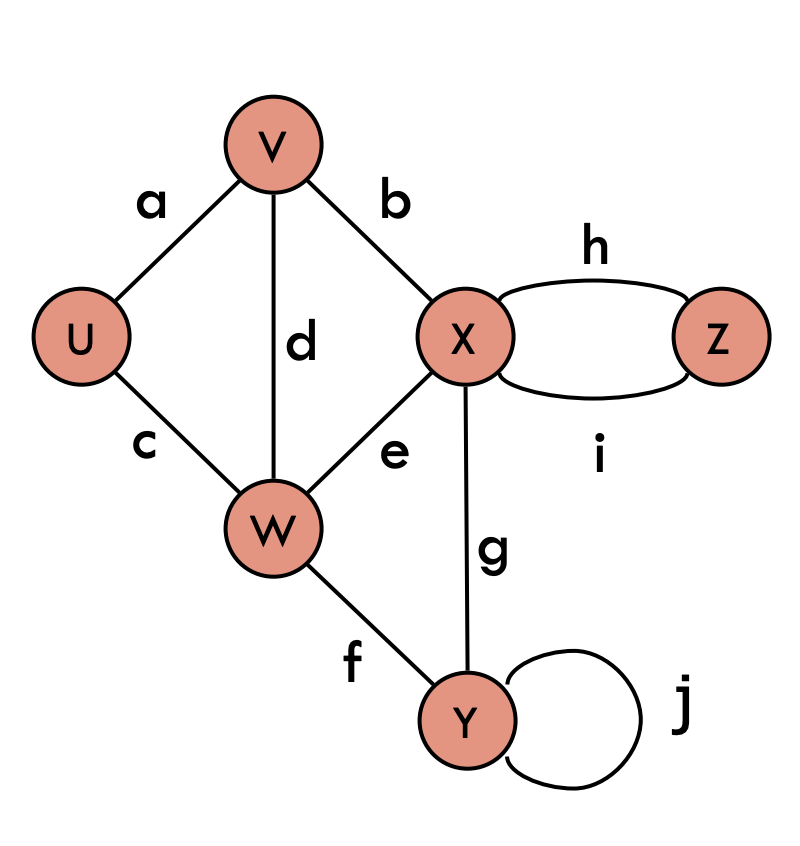
\includegraphics[width=\textwidth]{image16.png}
\end{minipage}

\subsection{Directed graphs}
\begin{minipage}[l]{0.6\textwidth}
  \begin{itemize}
    \item Edges go from tail to head (e.g., W is the tail of c and U its head)
    \item Out-degree is the number of edges out of a vertex (e.g., W has out-degree 2)
    \item In-degree is the number of edges into a vertex (e.g., W has in-degree 1)
    \item Parallel edges share tail and head (e.g., no parallel edge on the right)
    \item Self-loop have the same head and tail (e.g., X has a self-loop)
    \item Simple directed graphs have no parallel or self-loops, but are allowed to have antiparallel loops like f and a
  \end{itemize}
\end{minipage}
\begin{minipage}[r]{0.39\textwidth}
  \raggedleft
  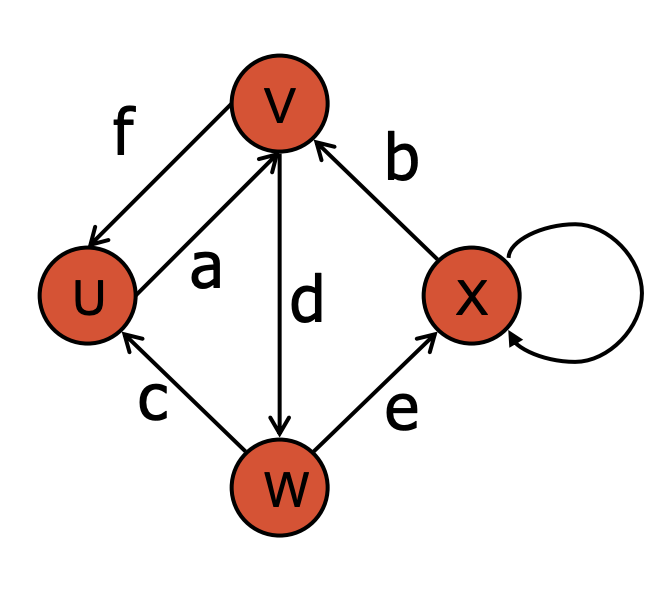
\includegraphics[width=\textwidth]{image17.png}
\end{minipage}

% Section 6  ----------------------------------------------------------------------------------------
\section{Weighted Graphs}
In a weighted graph, each edge has an associated numerical value, called the weight of the edge.
Edge weights may represent, distances, costs, etc.

\subsection{Shortest Paths}
Given an edge weighted graph and two vertices u and v, we want to find a path of minimum total weight between u and v, 
where the weight of a path is the sum of the weights of its edges.

\vspace{10pt}
\textbf{Properties:}
\begin{itemize}
  \item A subpath of the shortest path is itself the shortest path.
  \item There is a tree of the shortest paths from a start vertex to all the other vertices (Shortest path tree).
\end{itemize}
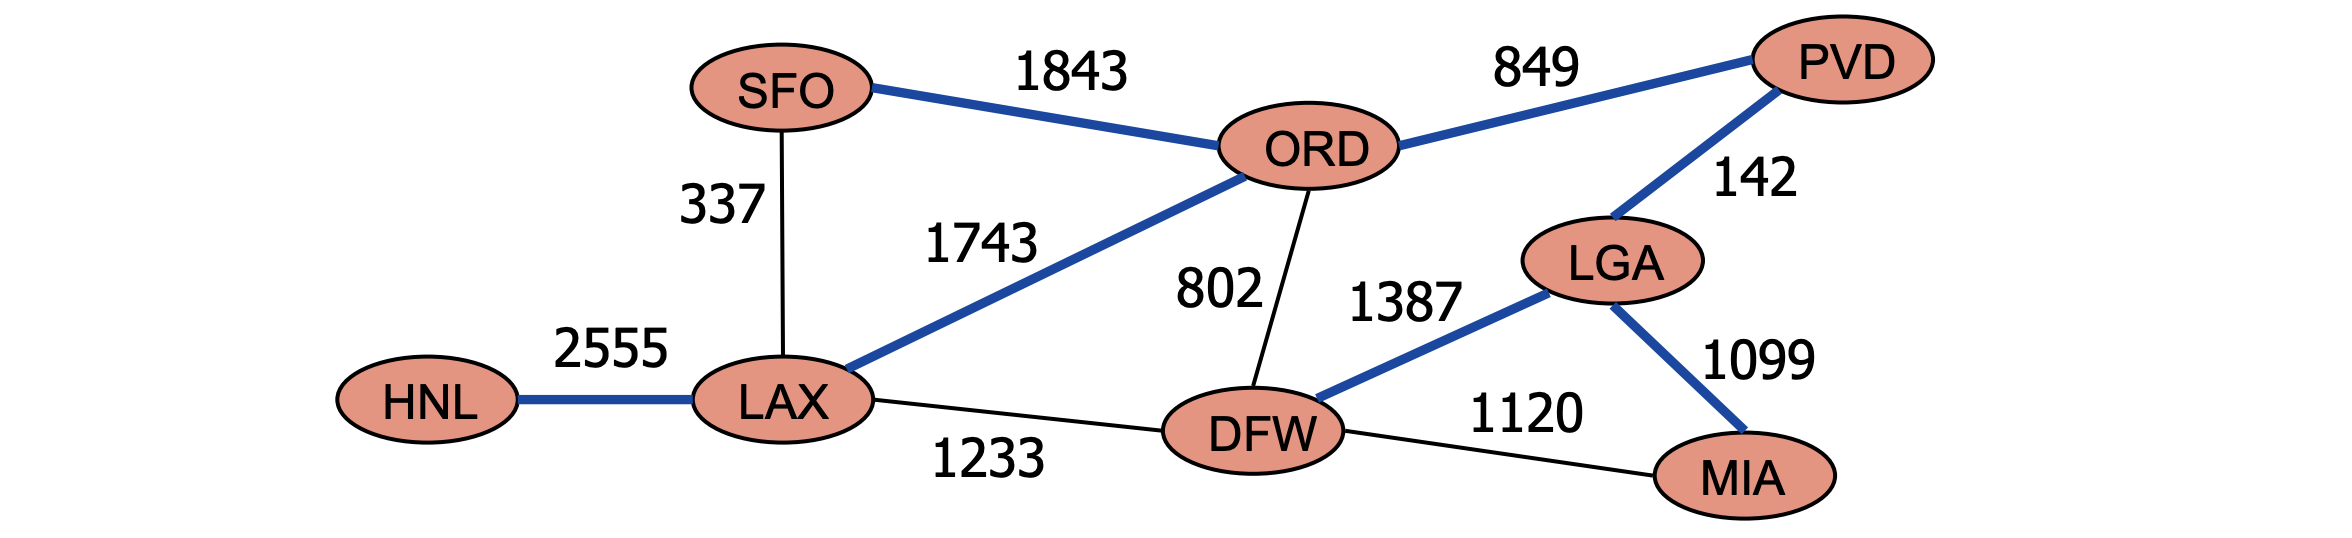
\includegraphics[width=\textwidth]{image18.png}

% Section 7  ----------------------------------------------------------------------------------------
\section{Dijkstra’s Algorithm}
\begin{minipage}[t]{0.5\textwidth}
  \textbf{Input:}
  \begin{itemize}
  \item Graph $G = (V, E)$.
  \item Edge weights $w : E \rightarrow R^+$.
  \item Start vertex $s$.
  \end{itemize}
  \textbf{Output:}
  \begin{itemize}
  \item Distance from $s$ to all $v$ in $V$.
  \item The shortest path tree rooted at $s$.
  \end{itemize}
  \textbf{Assumptions:}
  \begin{itemize}
  \item $G$ is connected and undirected.
  \item Edge weights are nonnegative.
  \end{itemize}
\end{minipage}
\begin{minipage}[t]{0.49\textwidth}
  \textbf{High level idea:}
  \begin{itemize}
  \item Maintain a distance estimate $D[v] \geq dist_w(s, v)$ for all $v$ in $V$.
  \item Keep track of a subset $S$ of $V$ such that $D[v] = dist_w(s, v)$ for all $v$ in $S$.
  \end{itemize}
  \textbf{Initially:}
  \begin{itemize}
  \item $D[s] = 0$.
  \item $D[v] = \infty$ for all $v$ in $V - s$.
  \end{itemize}
  \textbf{In each iteration we:}
  \begin{itemize}
  \item add to $S$ vertex $u$ in $V - S$ with smallest $D[u]$.
  \item update $D$-values for vertices adjacent to $u$.
  \end{itemize}
\end{minipage}

\subsection{Edge Relaxation}
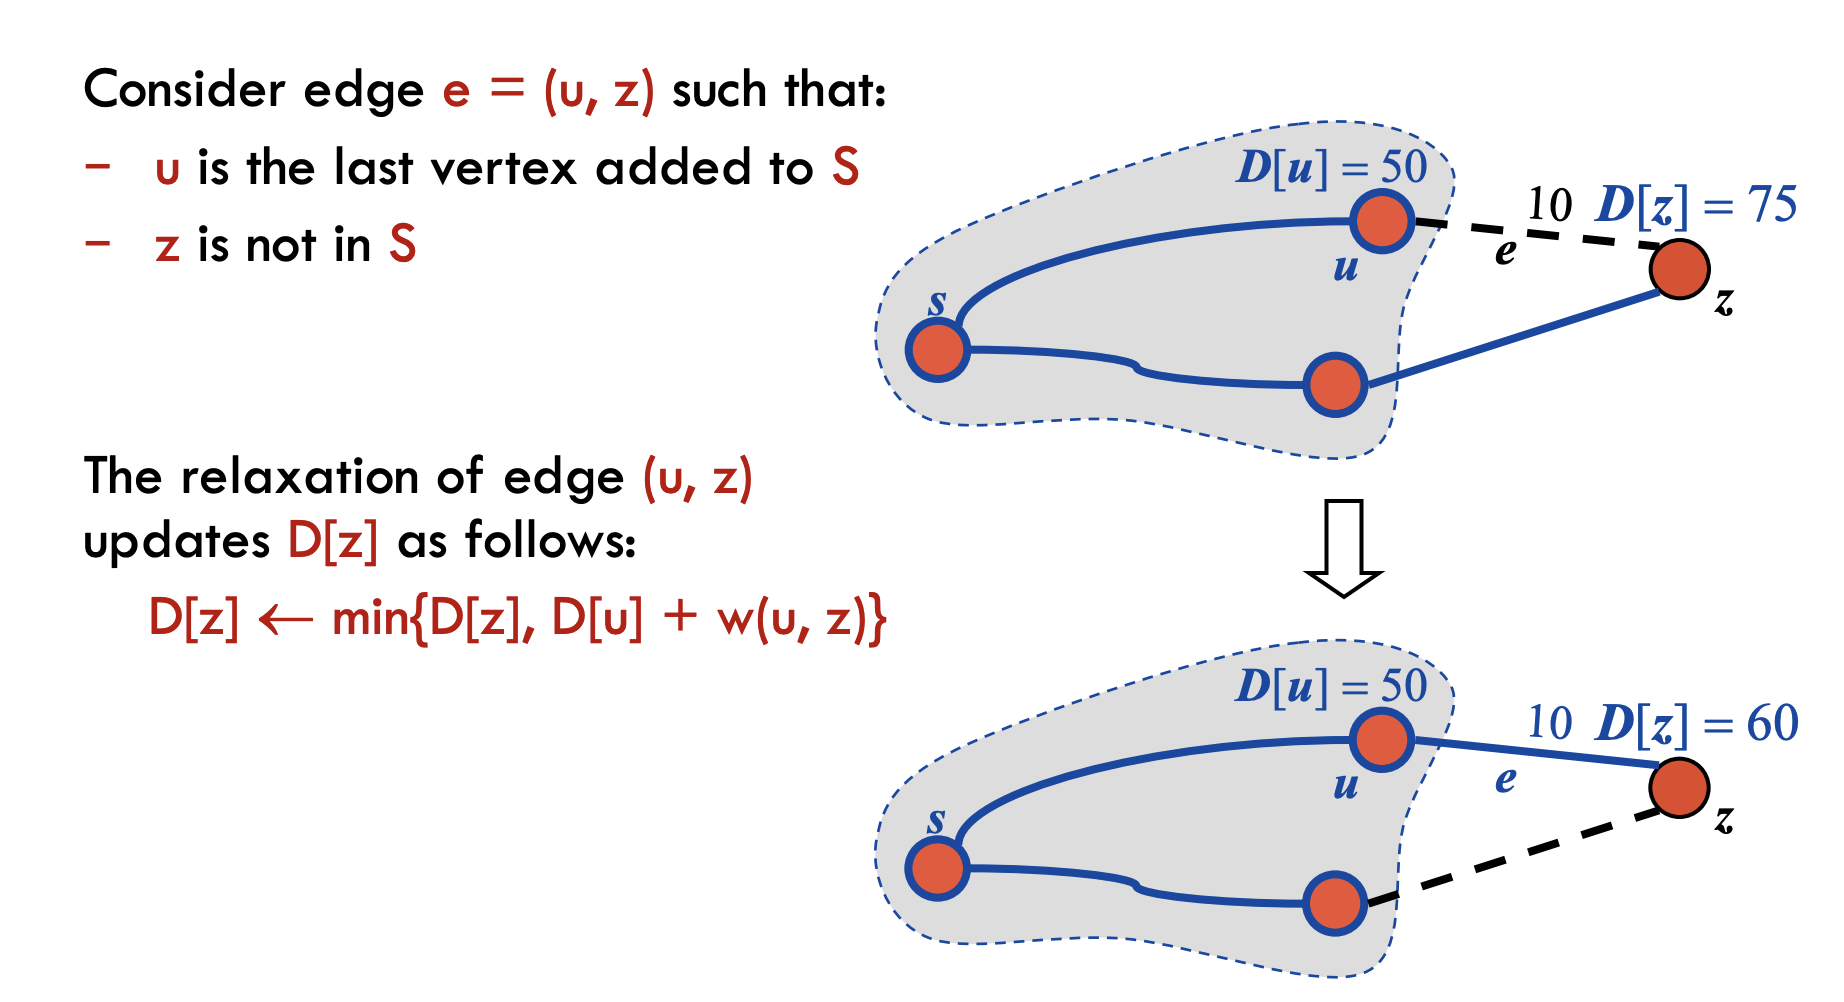
\includegraphics[width=\textwidth]{image19.png}

\subsection{Dijkstra’s Algorithm pseudocode}
\begin{pseudo}
  \I \DEF{Dijkstra}{G, w, s} \comment{Total run time is O(n + m log n)}
  \I \1 \for{v in G.vertices()} \comment{Set things up for Dijkstra: O(n)}
  \I \2 D[v] \assign $\infty$
  \I \2 parent[v] \assign null
  \I \1 D[s] \assign 0
  \I \1 Q \assign new PriorityQueue() for \{(v, D[v]) : v in V\} \comment{Key is depth estimate}
  \NL
  \I \1 \while{Q is not empty} \comment{iteratively add vertices to S: O(m log n)}
  \I \2 u \assign Q.removeMin()
  \I \2 \for{z in G.incidentEdges(u)} \comment{relax edges out of u: O(deg(u))}
  \I \3 \IF{D[z] > D[u] + w(u, z)}
  \I \4 D[z] \assign D[u] + w(u, z)
  \I \4 parent[z] \assign u
  \I \4 Q.update\_PriorityQueue(z, d[z])
  \I \1 \return{D, parent} \comment{dictionaries (vertex to shortest path from s) (vertex to parent) }
\end{pseudo}

\subsection{Dijkstra’s Algorithm Analysis}
\begin{itemize}
  \item Assuming the graph is connected (so $m \geq n-1$), the algorithm spends $O(m)$ time on everything except priority queue operations.
  \item The priority queue operations involve $n$ inserts, $m$ decrease\_key operations, and $n$ remove\_min operations.
  \item Using a binary heap for the priority queue, the total time complexity is $O(m \log n)$.
  \item Using a Fibonacci heap for the priority queue, the total time complexity is $O(m + n \log n)$, due to the $O(1)$ amortized time for decrease\_key operations.
\end{itemize}
\begin{center}
  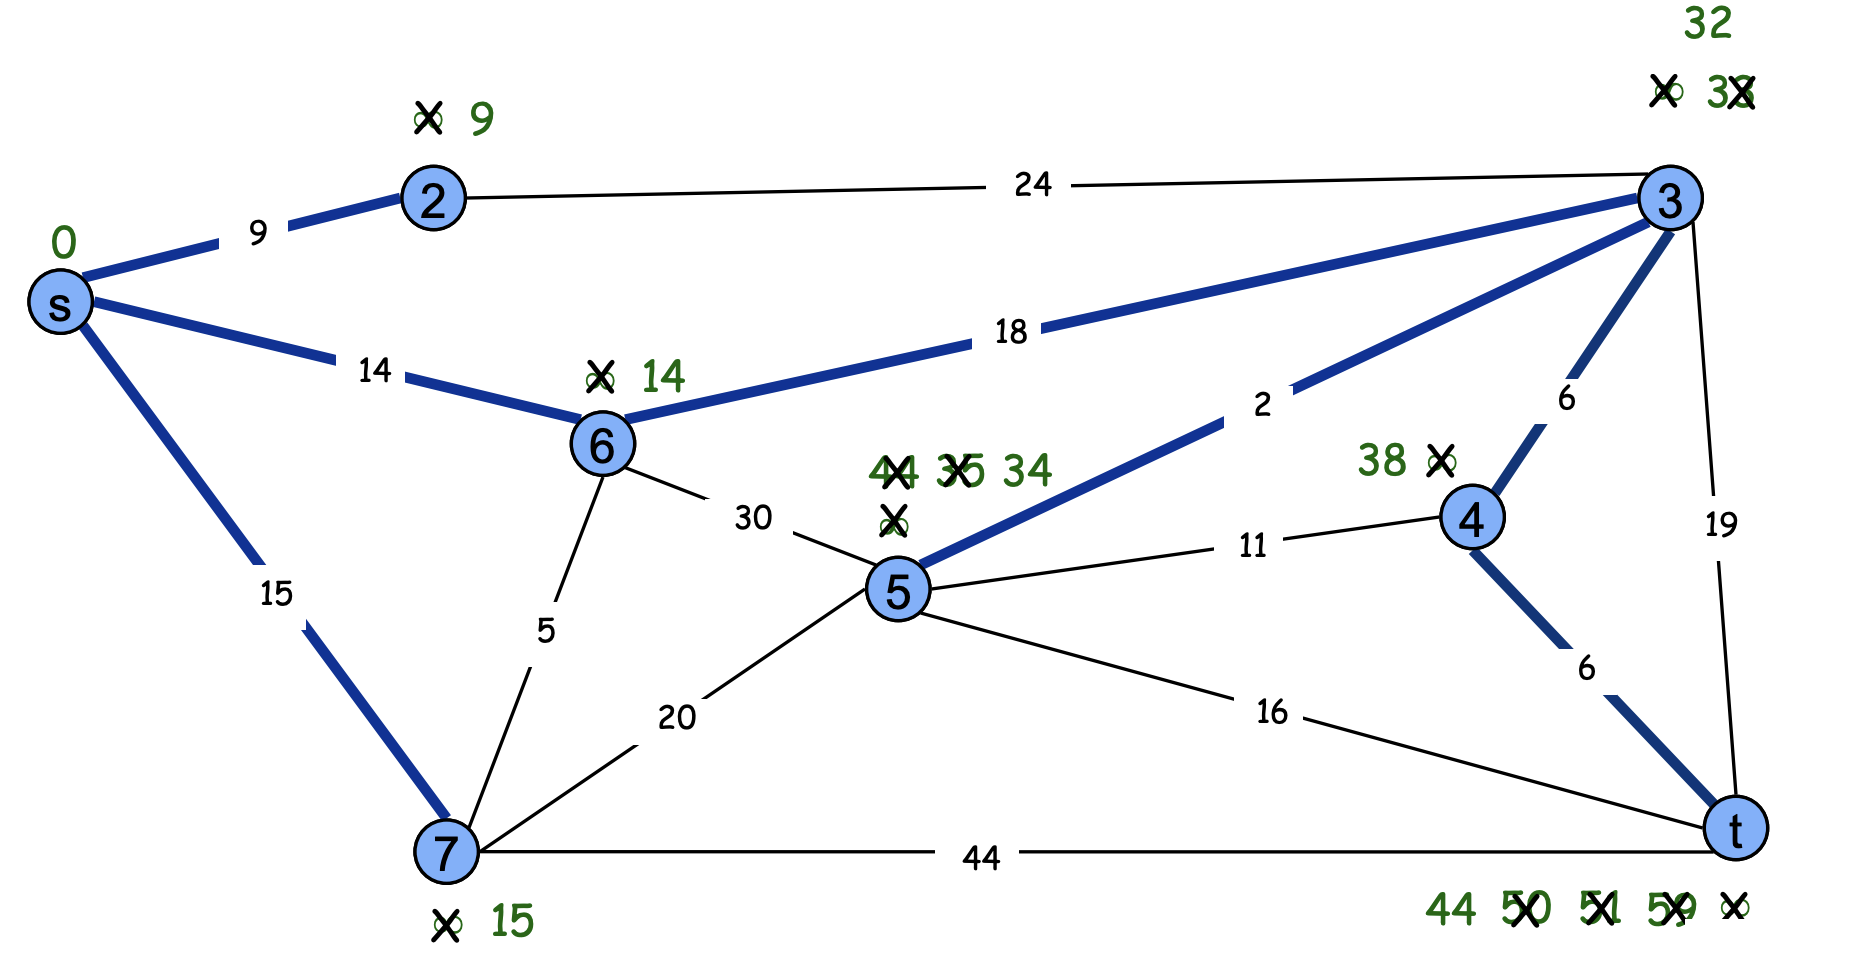
\includegraphics[width=0.9\textwidth]{image20.png}
\end{center}


\subsection{Correctness of Dijkstra’s Algorithm}
To prove Dijkstra’s correctness, we can use induction on the number of vertices visited by the algorithm. 
Let's denote the set of visited vertices as S and the set of unvisited vertices as V-S.

\vspace{10pt}
\textbf{Base case:}\\
At the start, the distance of the starting vertex s is 0, which is the correct shortest path distance from s 
to itself.

\vspace{10pt}
\textbf{Inductive step}\\
Assume that the algorithm maintains the correct shortest path distances for all vertices visited so far. Now 
we'll show that after visiting the next vertex u with the smallest distance among the unvisited vertices, 
the algorithm still maintains the correct shortest path distances for all visited vertices.
\begin{enumerate}
  \item Consider the shortest path P from the starting vertex s to u. We claim that P does not contain any other 
  unvisited vertices besides u. If P did contain another unvisited vertex w, the distance from s to w would be 
  shorter than the distance from s to u, which contradicts our choice of u as the closest unvisited vertex.
  \item After visiting u, we update the distance estimates for the neighbors of u. Since we've assumed that the 
  shortest path from s to u is correct, any updated distance estimate for a neighbor v of u will also be correct.
  This is because the new distance estimate for v takes into account the correct shortest path distance from s to u, 
  and the shortest path from s to v through u does not contain any other unvisited vertices (from point 1).
\end{enumerate}
By induction, Dijkstra's algorithm maintains the correct shortest path distances for all visited vertices. 
When all vertices are visited, the algorithm has computed the correct shortest path distances for the entire 
graph.

% Section 8  ----------------------------------------------------------------------------------------
\section{Minimum Spanning Trees}
Given a connected graph $G = (V, E)$ with real-valued edge weights $c_e$, an MST is a subset of the 
edges $T \subseteq E$ such that $T$ is a spanning tree whose sum of edge weights is minimized.
\begin{center}
  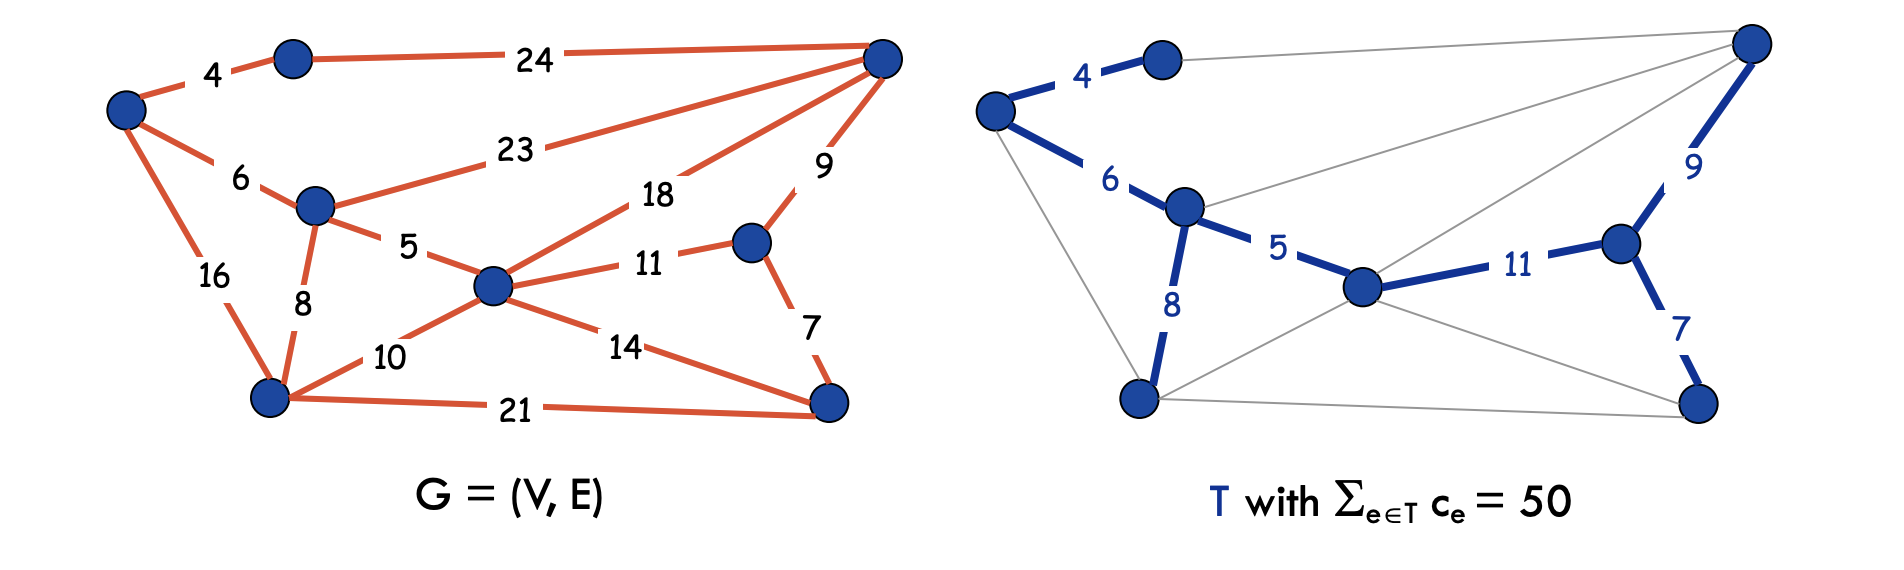
\includegraphics[width=0.8\textwidth]{image21.png}
\end{center}

\subsection{MST properties}
\textbf{Simplifying assumption:} All edge costs $c_e$ are distinct.

\vspace{10pt}
\textbf{Cut property:} Let S be any subset of nodes, and let e be the min cost edge with exactly one endpoint 
in S. Then the MST contains e.

\vspace{10pt}
\textbf{Cycle property:} Let C be any cycle, and let f be the max cost edge belonging to C. Then the MST does
not contain f.

\subsection{Cycles and Cuts}
\begin{center}
  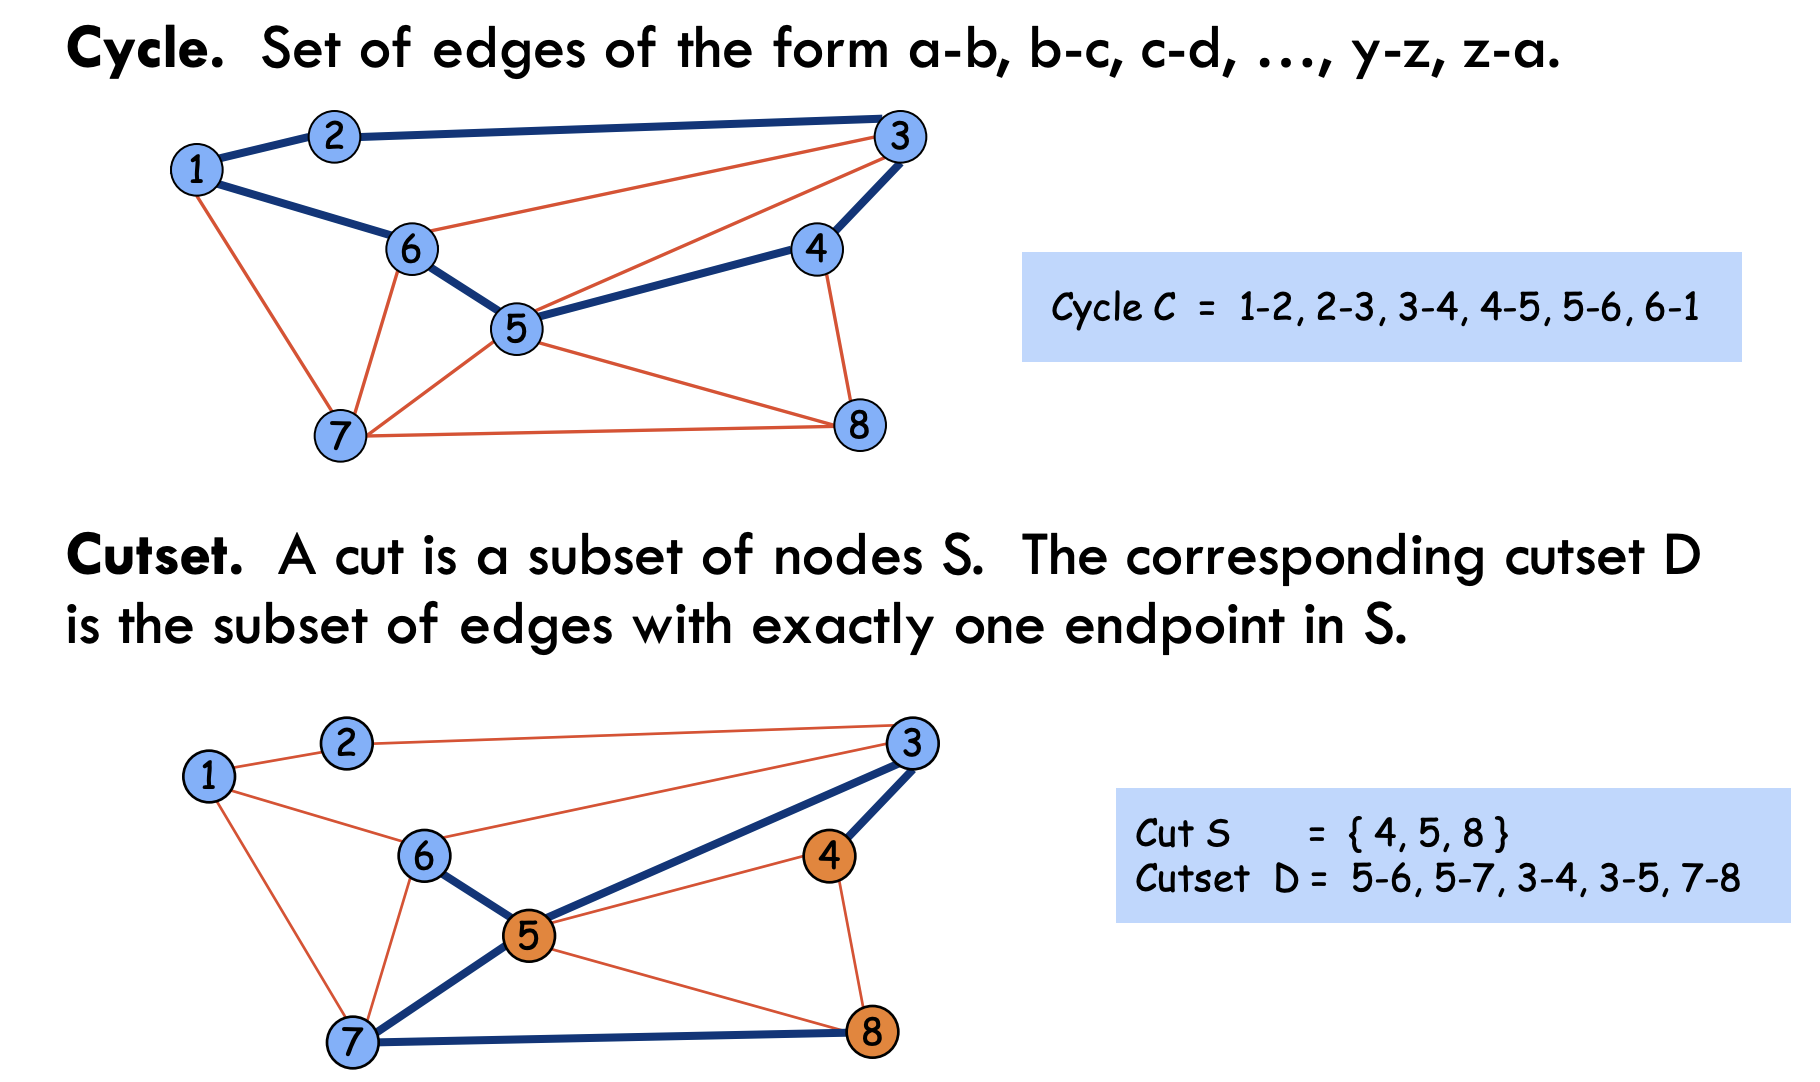
\includegraphics[width=0.8\textwidth]{image22.png}
  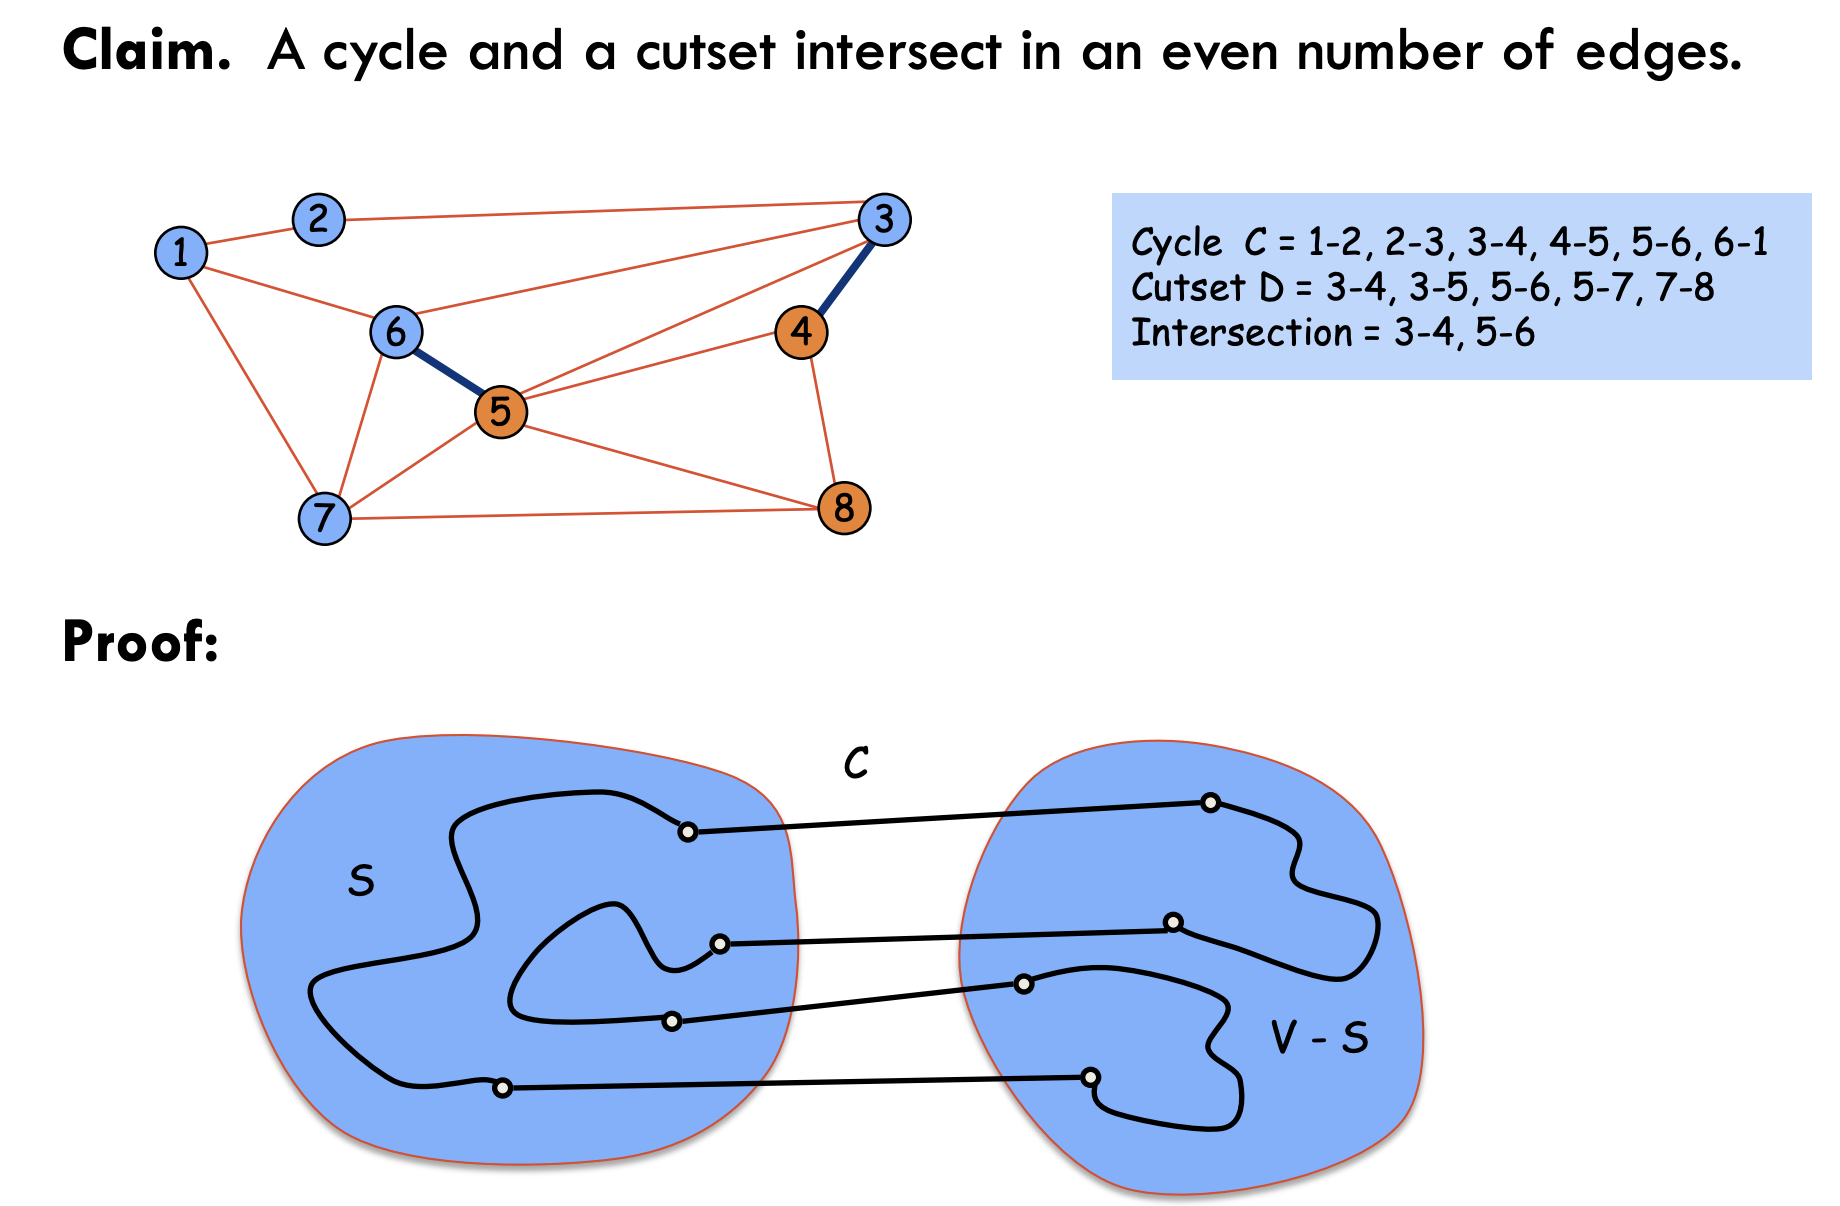
\includegraphics[width=0.8\textwidth]{image23.png}
\end{center}

% Section 9  ----------------------------------------------------------------------------------------
\section{Prim's Algorithm}
Every time we add an edge we follow cut property!
\begin{pseudo}
  \I \DEF{Prim}{G, c} \comment{C is the cost function. Total run time is O(n + m log n)}
  \I \1 \for{v in G.vertices()} \comment{Set things up for Prim: O(n)}
  \I \2 D[v] \assign $\infty$
  \I \2 parent[v] \assign null
  \I \1 u \assign any vertex in V
  \I \1 D[u] \assign 0
  \I \1 Q \assign new PriorityQueue() for \{(v, D[v]) : v in V\} \comment{Key is depth estimate}
  \I \1 S \assign []
  \NL
  \I \1 \while{Q is not empty} \comment{iteratively add vertices to S: O(m log n)}
  \I \2 u \assign Q.removeMin()
  \I \2 S.append(u)
  \I \2 \for{z in G.incidentEdges(u)} \comment{relax edges out of u: O(deg(u))}
  \I \3 \IF{z not in S and D[z] > c(u, z)}
  \I \4 parent[z] \assign u
  \I \4 decrease PriorityQueue d[z] to c(u, z)
  \I \1 \return{parent} \comment{parent is a dictionary that maps each vertex to its parent}
\end{pseudo}

\subsection{Prim's Algorithm Analysis}
Similar analysis to Dijkstra’s algorithm: O(m log n) using a heap and O(m + n log n) using Fibonacci heap.

\subsection{Dijkstra vs Prim and Kruskal}
MPT algorithms finds the minimum spanning tree of a connected, undirected graph, while Dijkstra's 
algorithm computes the shortest paths from a source vertex to all other vertices in a directed or 
undirected graph.
\begin{itemize}
  \item Shortest Path: The goal of finding the shortest path from a source vertex to all other vertices is 
  to identify the path with the minimum total weight between the source vertex and each of the other vertices 
  in the graph. The output of a shortest path algorithm (e.g., Dijkstra's algorithm) is a set of paths from the 
  source vertex to all other vertices in the graph.
  \item Minimum Spanning Tree: The goal of finding an MST is to create a tree that spans all vertices in the 
  graph while minimizing the sum of the edge weights. It connects all vertices without cycles and minimizes 
  the total edge weight. The output of an MST algorithm (e.g., Prim's or Kruskal's algorithm) is a tree that 
  spans all vertices in the graph with the minimum total edge weight.
\end{itemize}

\subsection{Correctness of Prim's Algorithm}
We'll prove that the tree constructed by Prim's algorithm is a minimum spanning tree (MST) by induction 
using the cut property.

\vspace{10pt}
\textbf{Base case:}\\
Initially, the set T is empty, which is a valid subset of the MST.

\vspace{10pt}
\textbf{Inductive hypothesis:} \\
Assume after k iterations, the set T contains k edges of the MST.

\vspace{10pt}
\textbf{Inductive step: } \\
In the (k+1)-th iteration, Prim's algorithm selects the lightest edge e crossing a cut C. We want to show that 
e is part of the MST.
\begin{enumerate}
\item If no MST M exists that contains edges in T but not edge e, then Prim's algorithm has already built the 
MST, and the proof is complete.
\item If an MST M exists, find another edge f in M connecting the same vertex sets as edge e. Adding f to the 
tree formed by Prim's algorithm creates a cycle crossing the cut C.
\item Edge e has the minimum weight among edges crossing the cut C, so the weight of e is less than or equal 
to the weight of f.
\item Construct a new spanning tree $M_1$ by replacing f with e in M. The weight of $M_1$ is less than or equal 
to the weight of M.
\item Since M is an MST and the weight of $M_1$ is no greater than M, $M_1$ is also an MST containing edge e.
\end{enumerate}
Thus, the edge e selected by Prim's algorithm in the (k+1)-th iteration is part of an MST. 
Therefore, by induciton, Prim's algorithm correctly constructs an MST.
\begin{center}
  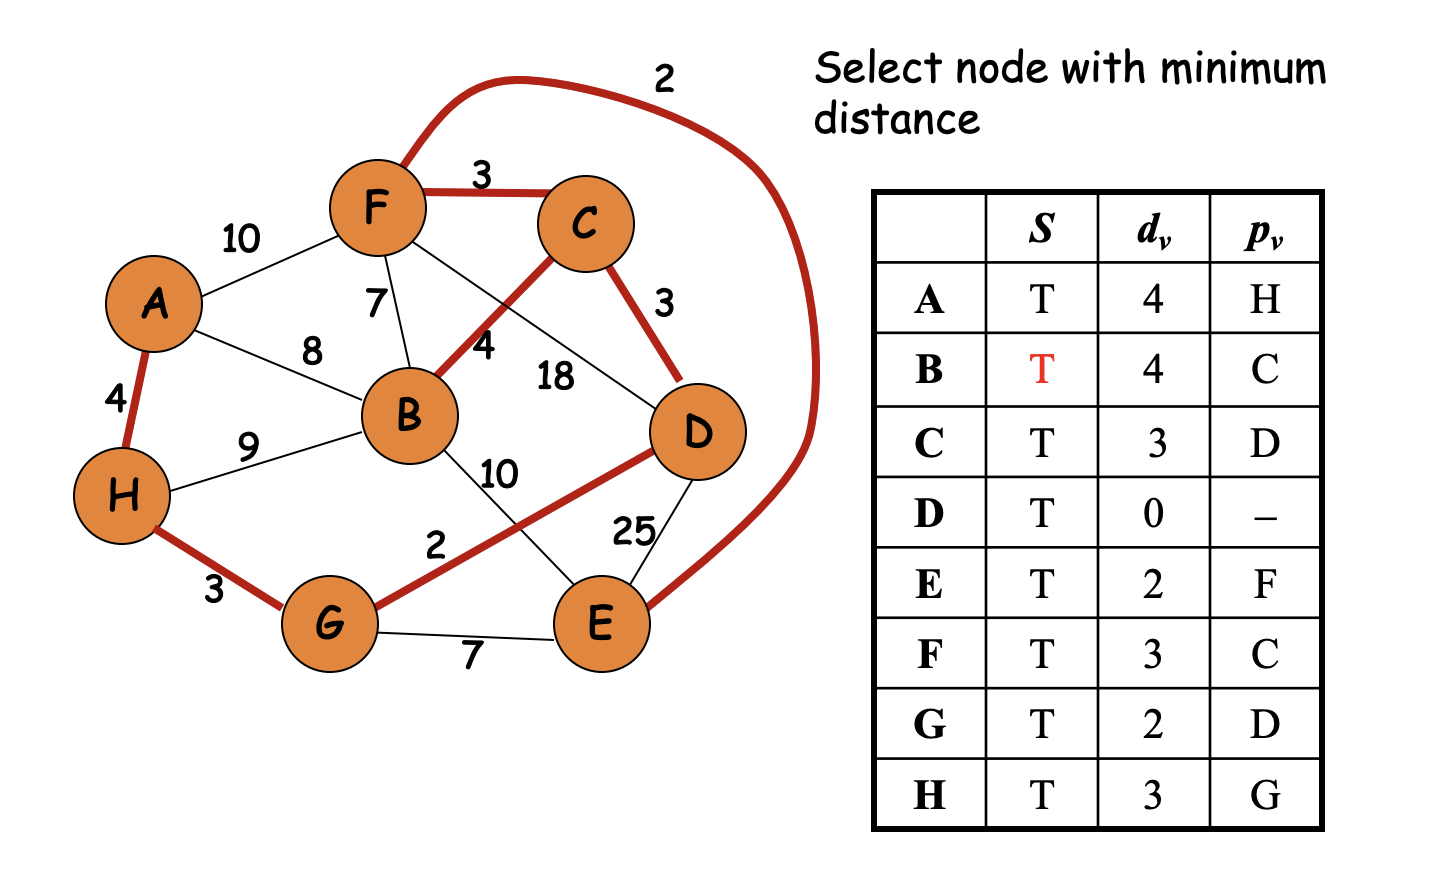
\includegraphics[width=0.75\textwidth]{image24.png}
\end{center}

% Section 10  ----------------------------------------------------------------------------------------
\section{Kruskal's Algorithm}
Kruskal's Algorithm works by examining the edges in ascending order of their weights and adding 
them to the MST if they do not create a cycle. Here's an expanded explanation of the algorithm:

\begin{enumerate}
  \item Sort all the edges in the graph in ascending order of their weights.
  \item Initialize the set $T$ as an empty set. This set will store the edges of the MST.
  \item For each edge $e$ in the sorted list, do the following:
  \begin{enumerate}
    \item Case 1 (Cycle): If adding edge $e$ to $T$ results in a cycle, discard $e$ according to the 
    cycle property. The cycle property states that in an MST, there cannot be any cycles. Discarding 
    $e$ ensures that the resulting MST remains acyclic.
    \item Case 2 (Cut): If adding edge $e$ to $T$ does not create a cycle, insert $e = (u, v)$ into 
    $T$ according to the cut property. The cut property states that for any partition of the graph's 
    vertices into two non-empty sets (a cut), the lightest edge crossing the partition must be included 
    in the MST. In this case, $S$ represents the set of nodes in the connected component of vertex $u$. 
    By adding edge $e$, we are connecting the components of vertices $u$ and $v$ while maintaining the 
    properties of an MST.
  \end{enumerate}
  \item Repeat step 3 for all edges in the sorted list.
  \item Once all edges have been processed, the set $T$ will contain the edges of the MST.
\end{enumerate}

\subsection{Union Find ADT}
Data structure defined on a ground set of elements A used to keep track of an evolving partition.
\begin{itemize}
  \item make\_sets(A): makes |A| singleton sets with elements in A. O(n)
  \item find(a): returns an id for the set element a belongs to. O(1)
  \item union(a,b): union the sets elements a and b belong to. O(1)
\end{itemize}

\includegraphics[width=\textwidth]{image25.png}

\subsection{Kurskal’s algorithm implementation}
\begin{pseudo}
  \I \DEF{Kruskal}{G, c} \comment{c is the cost function. Total run time is O(m log n)}
  \I \1 sort E by increasing c-value order \comment{O(m log m)}
  \I \1 T \assign []
  \I \1 comp \assign make\_sets(V) \comment{O(n)}
  \I \1 \for{e in E} \comment{O(m)}
  \I \2 \IF{comp.find(e.u) != comp.find(e.v)}
  \I \3 T.append(e)
  \I \3 comp.union(e.u, e.v)
  \I \1 \return{T}
\end{pseudo}

\subsection{Lexicographic Tiebreaking}
To remove the assumption that all edge costs are distinct, we can perturb all edge costs by tiny amounts 
to break any ties. The impact of this perturbation is minimal because Kruskal and Prim's algorithms only 
interact with costs through pairwise comparisons. If the perturbations are sufficiently small, the MST with 
perturbed costs will be the same as the MST with the original costs. For instance, if we assume that all 
costs are integral, adding i/$n^2$ to each edge e\_i would not significantly alter the MST. Under these 
perturbed weights, any MST found would still be an MST under the original weights, ensuring that 
the algorithms continue to function correctly despite the small changes in edge costs.
\end{document}